\chapter{A verification of the axisymmetric model: model of a naked jet}\label{chapter6}
%%%%%%%%%%%%%%%%%%%%%%%%%%%%%%%%%%%%%%%%%%%%%%%%%%%%%%%%%%%%%%%%%%%%%%%%
% 
%												Further implication of axisymmetric model 
%
%%%%%%%%%%%%%%%%%%%%%%%%%%%%%%%%%%%%%%%%%%%%%%%%%%%%%%%%%%%%%%%%%%%%%%%%
%\section{A verification of the axisymmetric model: naked jet}
The simulations of jets propagating into the cluster atmosphere conducted in the previous two chapters typically evolve to an extent of around 50 kpc, which is the extent of the simulation domain. The jet evolution occurs over a timescale of approximately 20~Myr. While the shock structures in the jet, the turbulent transition of the jet, and global structures, e.g. the turbulent backflows in the cocoon and forward shock of the bubble, are well captured in the simulations, the physical simulation time is less than the age of the source, which is approximately \noteA{age of source}. It is possible, therefore, that the properties of the flow adjacent to the simulated jet stream are not representative of the medium the real jet stream is engulfed in. For example, the simulated jet may be strongly affected by the backflow generated as the jet propagates within this restricted domain.

The purpose of this chapter is, thus, to ascertain whether the shock positions seen in the simulations are affected by the backflow originating from the head of the jet down along the jet stream. To this end, I look at the evolution of the shock positions with time, and also perform a simulation of an unbounded jet -- a jet spanning the entire domain and not bounded by a termination shock. I refer to such an jet as a ``naked jet''. This is more representative of conditions in the inner regions of an evolved radio source, such as that of Hydra A. The fact that the shock positions are not affected by the backflowing ambient plasma, will reassure us that the results presented of in the previous chapter are applicable to the inner Hydra A jet during later stages of its evolution.

%The simulations of jets propagating into the cluster atmosphere conducted above typically evolve to an extent of 50 kpc, as restricted by the simulation domain, over a timescale of approximately 20~Myr. While the shock structures in the jet, the turbulent transition of the jet, and global structures, e.g. the turbulent backflows in the cocoon and forward shock of the bubble, are well captured, the simulation time is less than the age of the source. I therefore need to ascertain whether the shock positions seen in the simulations are likely to approach asymptotic values with time. To this end I look at the evolution of the shock positions with time, and also perform a simulation of an unbounded jet -- a jet spanning the entire domain and not bounded by a termination shock, which is more representative of conditions in the inner regions of an evolved radio source, such as that of Hydra A. 

\subsection{Simulation results} \label{s:jet_stream}
\begin{figure}
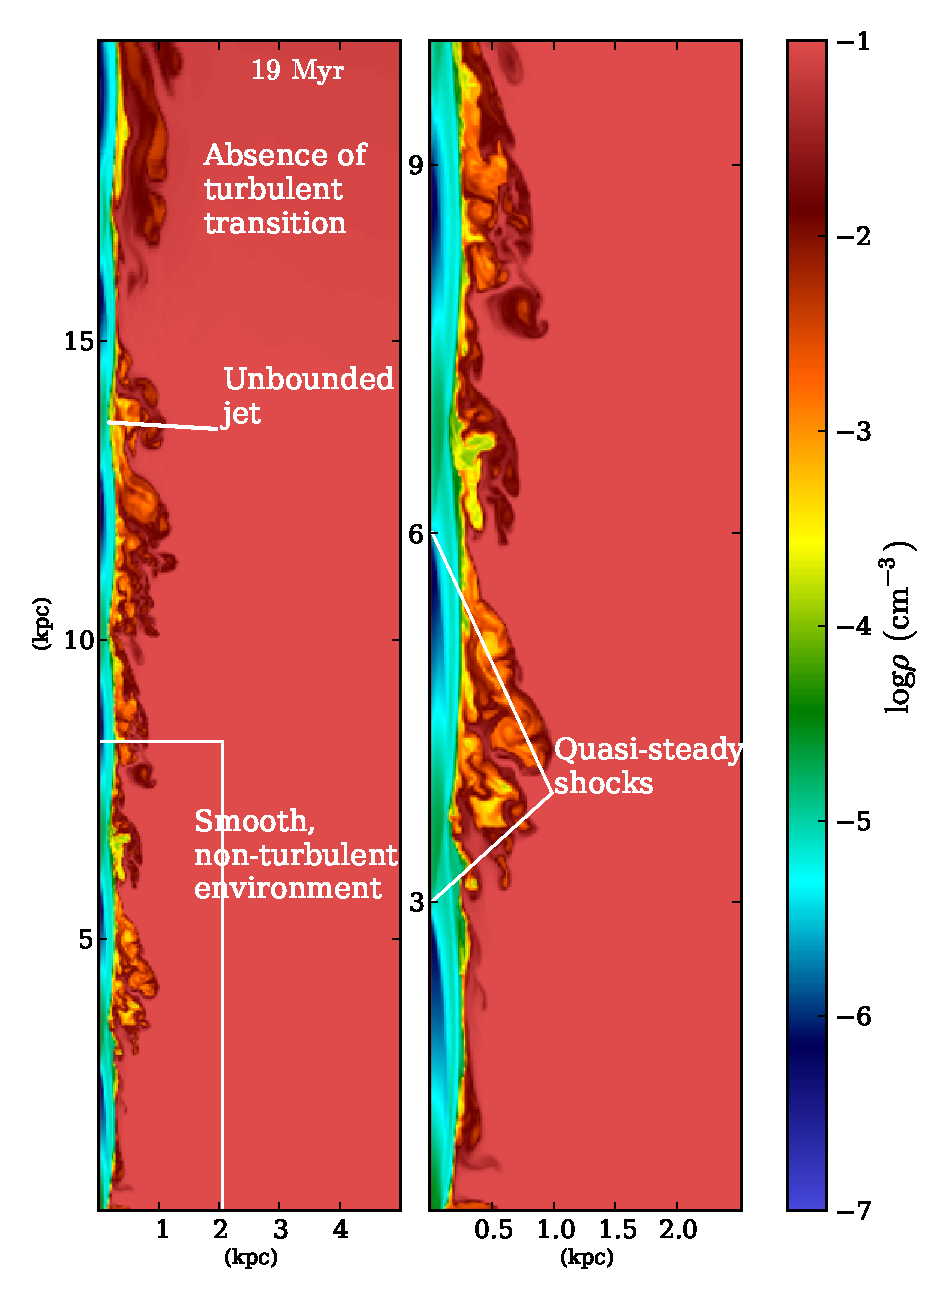
\includegraphics[width=\linewidth]{njm.eps}
\caption{Logarithmic density image of a snapshot in during the simulation of the interaction of an unbounded ``naked'' jet with a non-turbulent ICM. The shock positions are almost time-independent as the jet expands and reconfines multiple times before escaping through the top boundary. No transition to turbulent flow is observed. The right panel is a close-up of the central region marked with a box in the left panel. In both panels the physical scales are in units of kpc.}
\label{f:u_jet}
\end{figure}

\begin{figure}
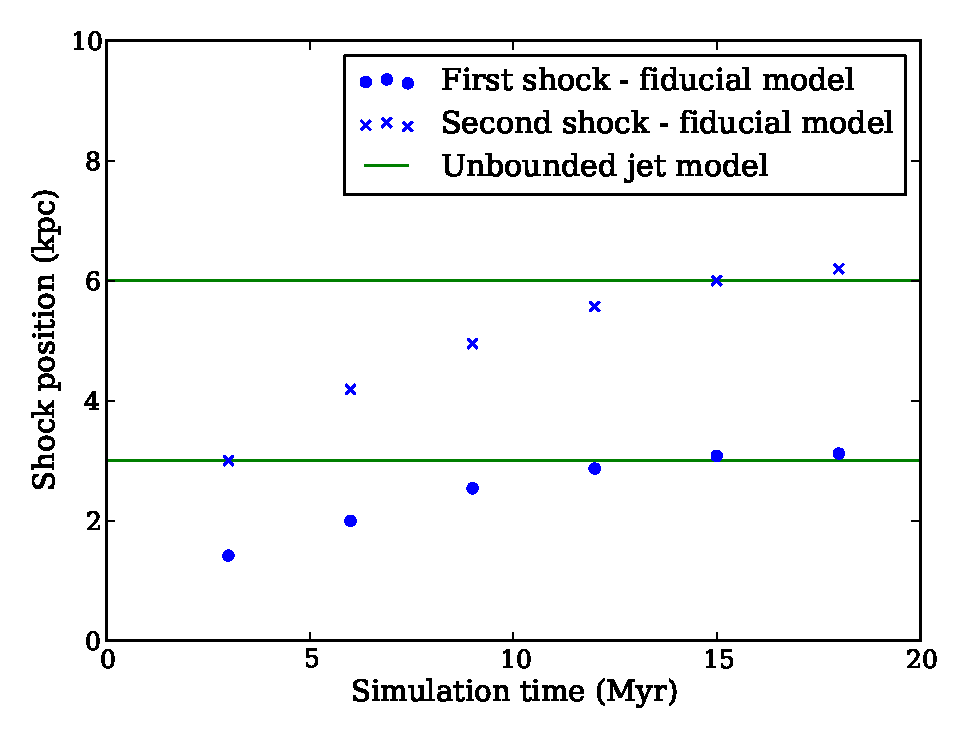
\includegraphics[width=\linewidth]{nse.eps}
\caption{Evolution of the reconfinement shock positions with time for model Cvii. The circles and crosses represent the first and second shock locations, respectively. The horizontal lines mark the shock positions obtained in the simulation of an unbounded ``naked'' jet using the same parameters as those in model Cvii.}
\label{f:c_vs_n}
\end{figure}



The simulation of an unbounded ``naked '' jet is an axis-symmetric relativistic hydrodynamic simulation.  I set up the the jet inlet with the same jet parameters and geometry as in run Cv, but I also initiate the full extent of a jet column spanning the length of the domain along the jet axis at the start of the simulation. The radial profiles for the hot atmosphere, the boundary conditions, and the numerical scheme are the same as those in the simulations presented in Chapter~\ref{chapter5}.

Since the jet is initially overpressured, it expands, then contracts, sending a nearly axis-symmetric shock wave into the ambient medium, and forming reconfinement shocks along the jet axis. Kelvin-Helmholtz instabilities develop in the shear layer between the jet and the ambient medium, but other than the initial adjustment, the flow in the entire simulation box is broadly time-independent. Without a jet backflow, a turbulent cocoon does not develop.

Figure~\ref{f:u_jet} shows the features developed by a naked jet model at time $t=19$ Myr. The right panel shows a closeup of the in central $5\times20$ kpc region. The jet is embedded in a relatively steady ambient medium exhibits the first two reconfinement shocks at approximately 3 and 6 kpc.

Simulations of naked jets allow us to measure the quasi-steady reconfinement shock positions because, in the absence of a turbulent cocoon, the global structure of the flow in the simulation domain and the pressure field of the medium surrounding the jet remain fairly steady. Thus, the naked jet streams, as presented in the simulations here, can be thought of the state of the inner jet stream for a source that has evolved to much larger spatial extents than the region contained in the simulation box, largely unperturbed by the distant turbulent cocoon. One restriction is, of course, that the nearly steady state structure of the ambient hot atmosphere would not obtain beyond its cooling time.

Figure~\ref{f:c_vs_n} shows the evolution of the first (circles) and second (crosses) shock positions for model Cv, respectively, as a function of time. The shock positions increase with time, but appear to asymptote to values very close to 3 and 6 kpc, respectively. The locations of the two reconfinement shocks in the naked jet model are also shown in Fig.~\ref{f:c_vs_n} with two horizontal lines. These shock locations agree with the asymptotic values of the shock position in run Ciii. 


Simulations of unbounded naked jets are useful for accurately measuring nearly time-independent positions of shocks in a jet, provided the top outflowing boundary is not affecting the structure of the jet. However, these models are not useful in explaining other important features of the Hydra A northern jet, in particular, the turbulent transition of the jet and the formation of the plume structure. As we see in the naked jet simulation the deceleration through the biconical shocks and the entrainment in the shear layer is insufficient to produce a turbulent transition of the jet stream to a plume. From this, I surmise that the ram pressure of the turbulent back flow in the cocoon plays an important role in further decelerating and disrupting of the jet. We see this phenomenon, at least qualitatively, in the simulations of an evolving jet, in which the jet is surrounded by a cocoon of entrained, turbulent, backflowing plasma, and is clearly affected by the surrounding flow. 

